\begin{flushleft}
\section{\LARGE{Prezentacja}}
\end{flushleft}

\begin{flushleft}
    \subsection{\Large{Logowanie}}
    \hspace{5mm}Uruchomiwszy aplikację, użytkowniku wyświetla się okno logowania:
    \begin{figure}[H]
	\begin{center}
	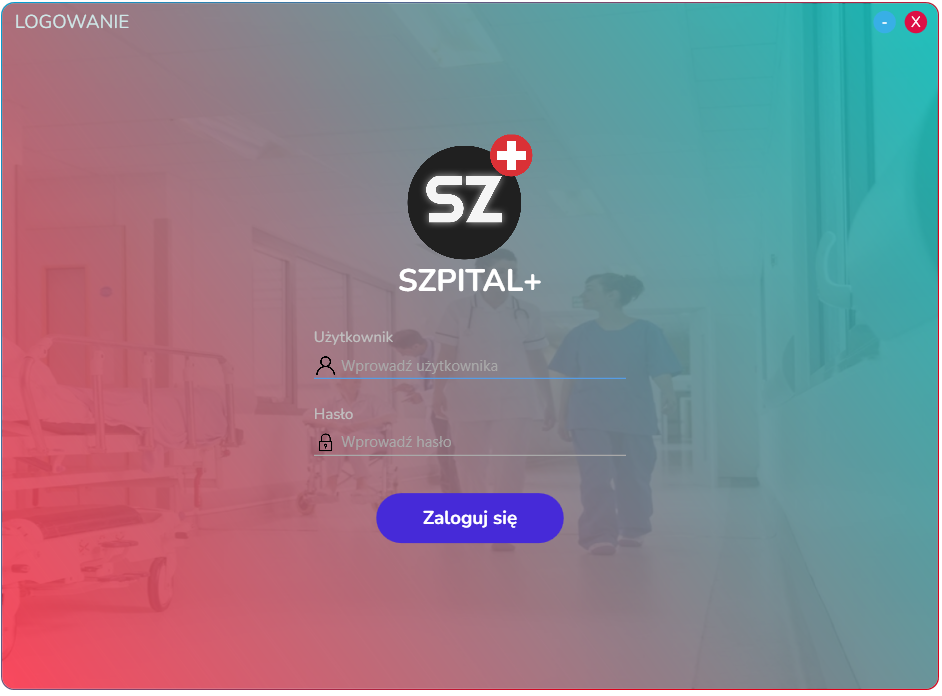
\includegraphics[height=7cm]{images/log_widok.png}
        \caption{Okno logowania}
        \label{fig:okn_log}
	\end{center}
    \end{figure}
    \hspace{5mm}W tym oknie został przerobiony górny standardowy panel aplikacji windows. Rozmiar okna 750x550px. Także tło oraz granica zrobione z gradientu. Okno jest trochę zaokrąglone. Po wprowadzeniu danych i naciśnięciu przycisku \textquotedbl Zaloguj się\textquotedbl{} klasa statyczna DbContext sprawdza czy użytkownik istnieje i czy hasło jest poprawne za pomocą polecenia SQL. W przypadku gdy użytkownik poda błędne dane DbContext rzuca wyjątek \textquotedbl UserIdentifyException\textquotedbl{} który jest łapany w LoginCommand, skąd wypisuje się komunikat.
    \begin{figure}[H]
	\begin{center}
	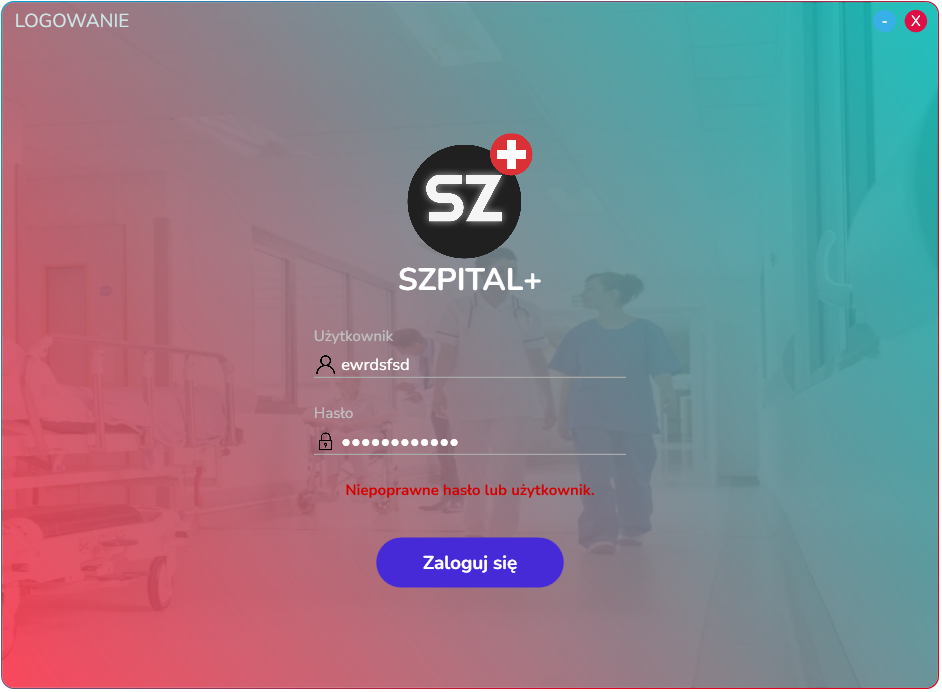
\includegraphics[height=8cm]{images/niep_uzyt.png}
        \caption{Wprowadzenie błędnych danych do logowania}
        \label{fig:okn_log}
	\end{center}
    \end{figure}
    \hspace{5mm}Jeśli użytkownik istnieje i hasło jest poprawne —logujemy się do aplikacji.
    \begin{figure}[H]
    \centering
    \subfigure{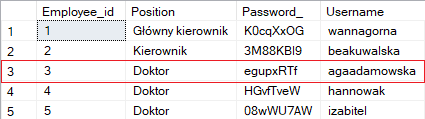
\includegraphics[width=0.7\textwidth]{images/istn_uzyt.png}} 
    \subfigure{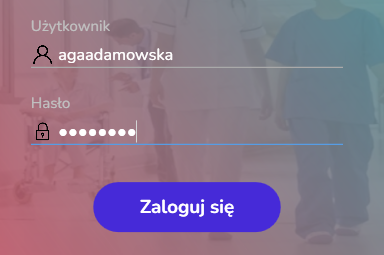
\includegraphics[width=0.3\textwidth]{images/rand_uzyt1.png}}
    \subfigure{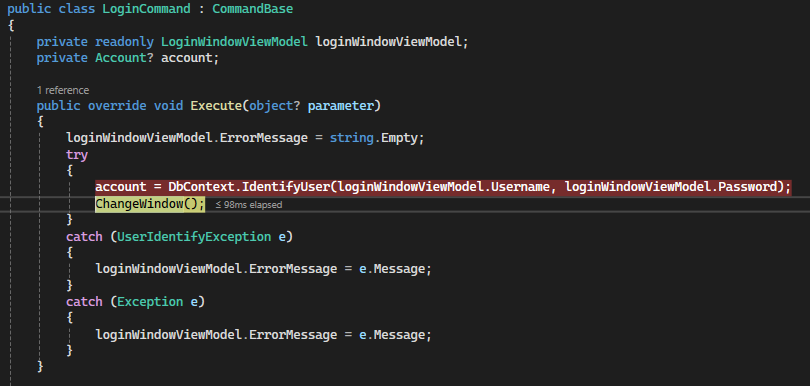
\includegraphics[width=0.5\textwidth]{images/log_kom_exe.png}}
    \caption{Logowanie (DbContext nie rzucił wyjątku)}
    \label{fig:popr_log}
    \end{figure}
    \subsection{\Large{Główne okno}}
    \hspace{5mm}MainWindow(Okno główne) składa się z trzech części:
    \begin{figure}[H]
	\begin{center}
	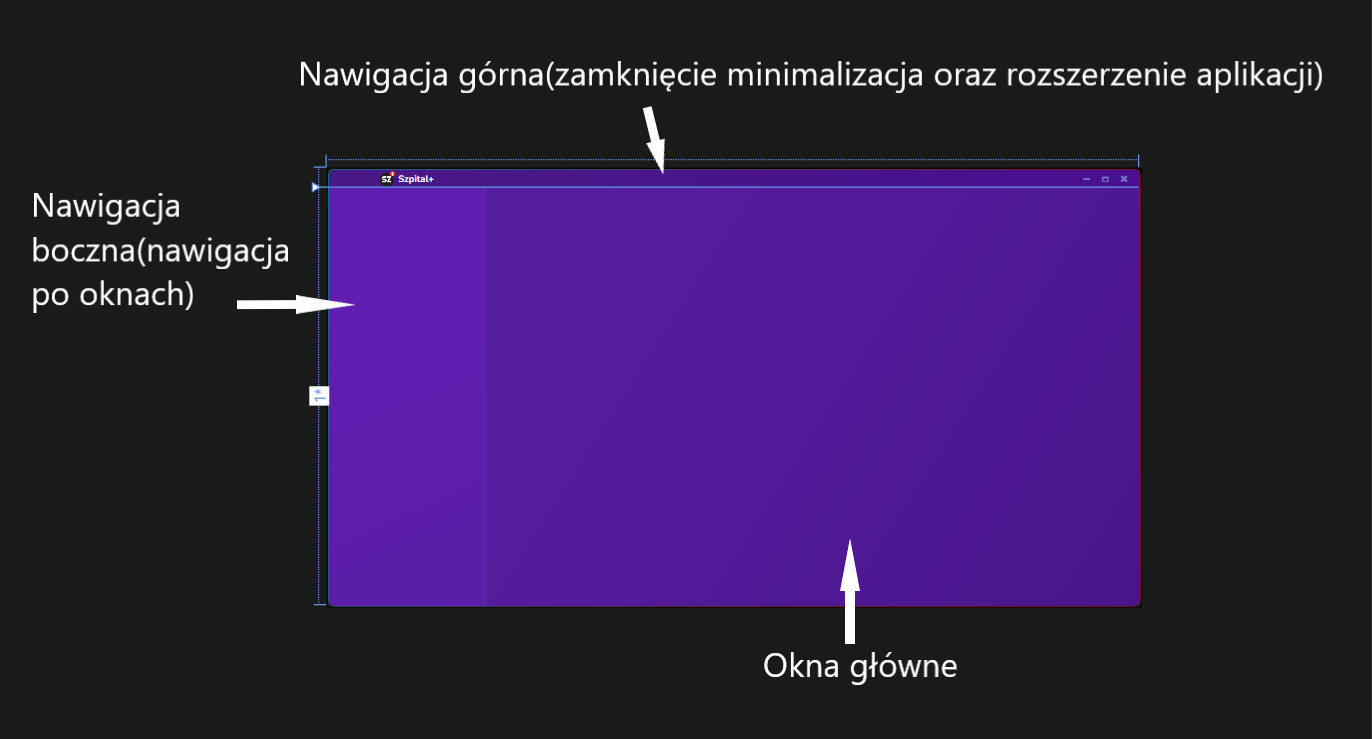
\includegraphics[height=8cm]{images/mainwindow.png}
        \caption{Główne okno}
        \label{fig:okn_glow}
	\end{center}
    \end{figure}
    \hspace{5mm}Aplikacja pobiera dane z bazy i ze względu na to, na jakim stanowisku pracuje użytkownik, wykorzystuje jeden z szablonów dotyczący jego posady żeby stworzyć nowy wygląd nawigacji bocznej.
    \begin{figure}[H]
	\begin{center}
	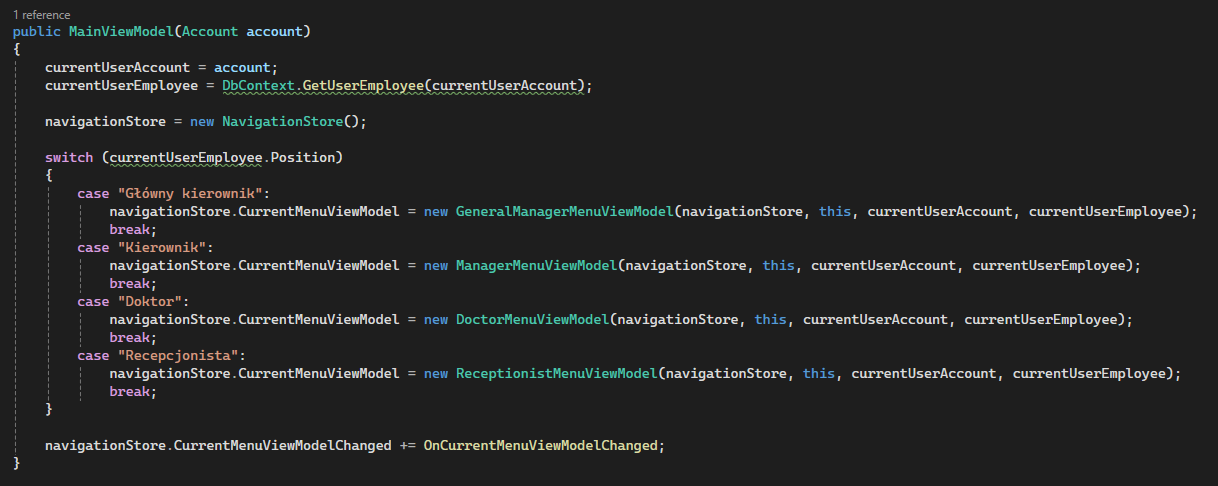
\includegraphics[height=5cm]{images/mainviewmodel_const.png}
        \caption{Pobieranie stanowiska użytkownika i przypisanie nowego wyglądu}
        \label{fig:main_vm_const}
	\end{center}
    \end{figure}
    \hspace{5mm}Na przykład do aplikacji został zalogowany Recepcjonista.
    Wtedy wygląd jego aplikacji będzie następny(także aplikacja sprawdza jaki zwrot wykorzystać na pulpicie ze względu na płeć osoby):
    \begin{figure}[H]
	\begin{center}
	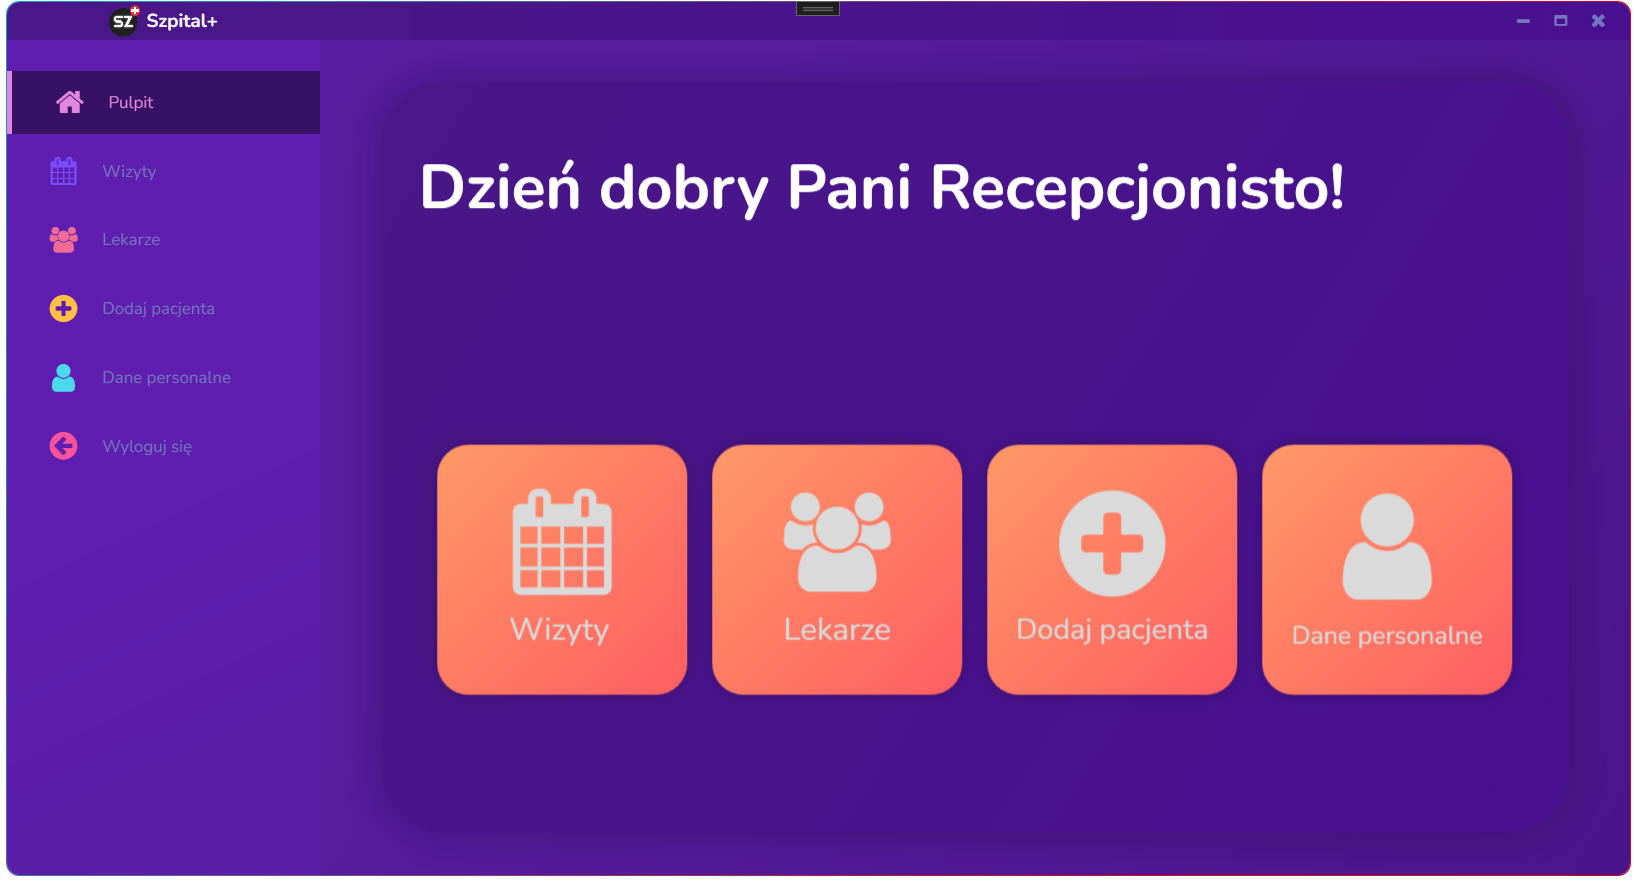
\includegraphics[height=7cm]{images/recep_view.png}
        \caption{Wygląd aplikacji recepcjonisty(Katarzyna Pabiniak)}
        \label{fig:recep_view}
	\end{center}
    \end{figure}
    \begin{figure}[H]
        \begin{center}
	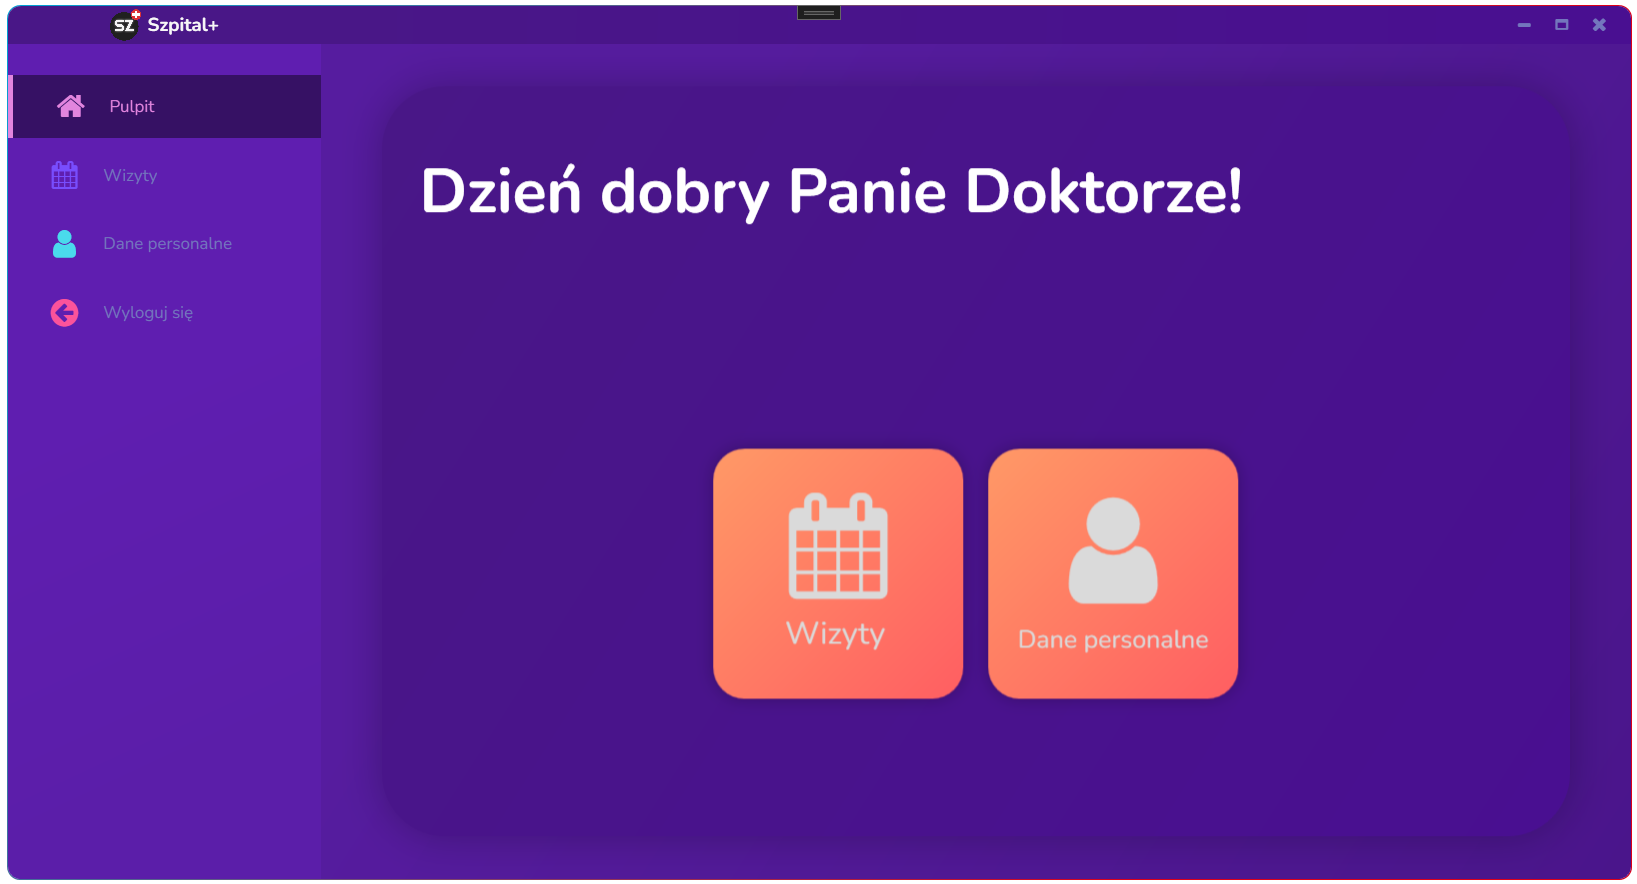
\includegraphics[height=7cm]{images/doktor_view.png}
        \caption{Wygląd aplikacji doktora(Filip Jabcoń)}
        \label{fig:doktor_view}
	\end{center}
    \end{figure}
    \hspace{5mm}Każdy klient na panelu nawigacyjnym bocznym ma przyciski: pulpit(okno z nawigacją), dane personalne(dane o użytkowniku), wyloguj się(wylogowanie z systemu i wracanie do okna logowania).
    \subsection{\Large{Dane personalne}}
    \begin{figure}[H]
    \centering
    \subfigure{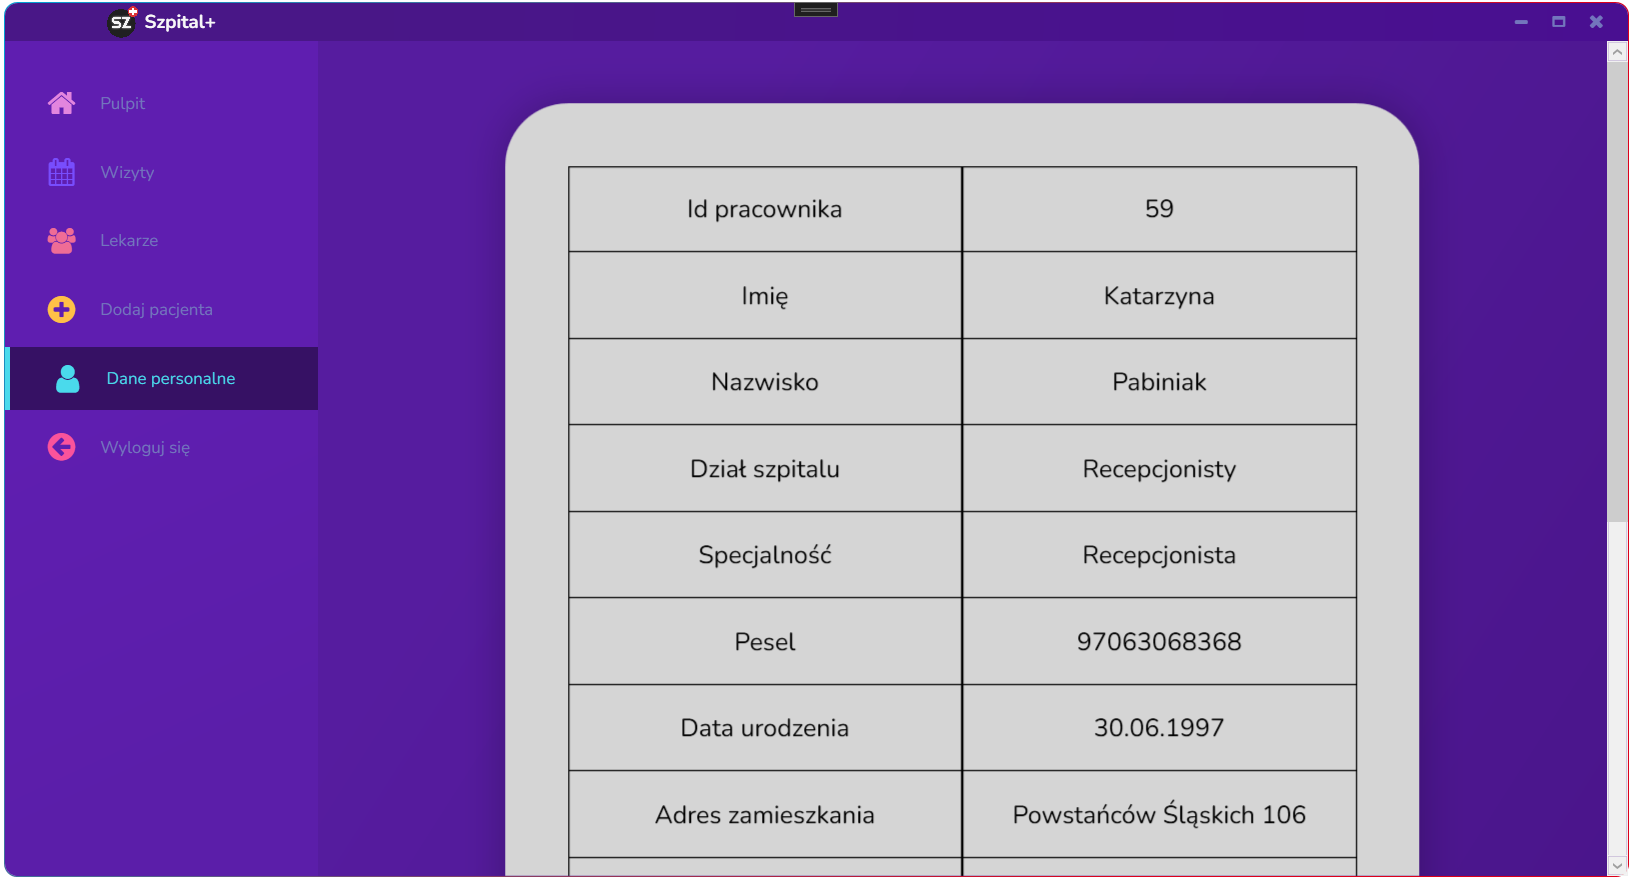
\includegraphics[width=0.7\textwidth]{images/dane_person1.png}} 
    \subfigure{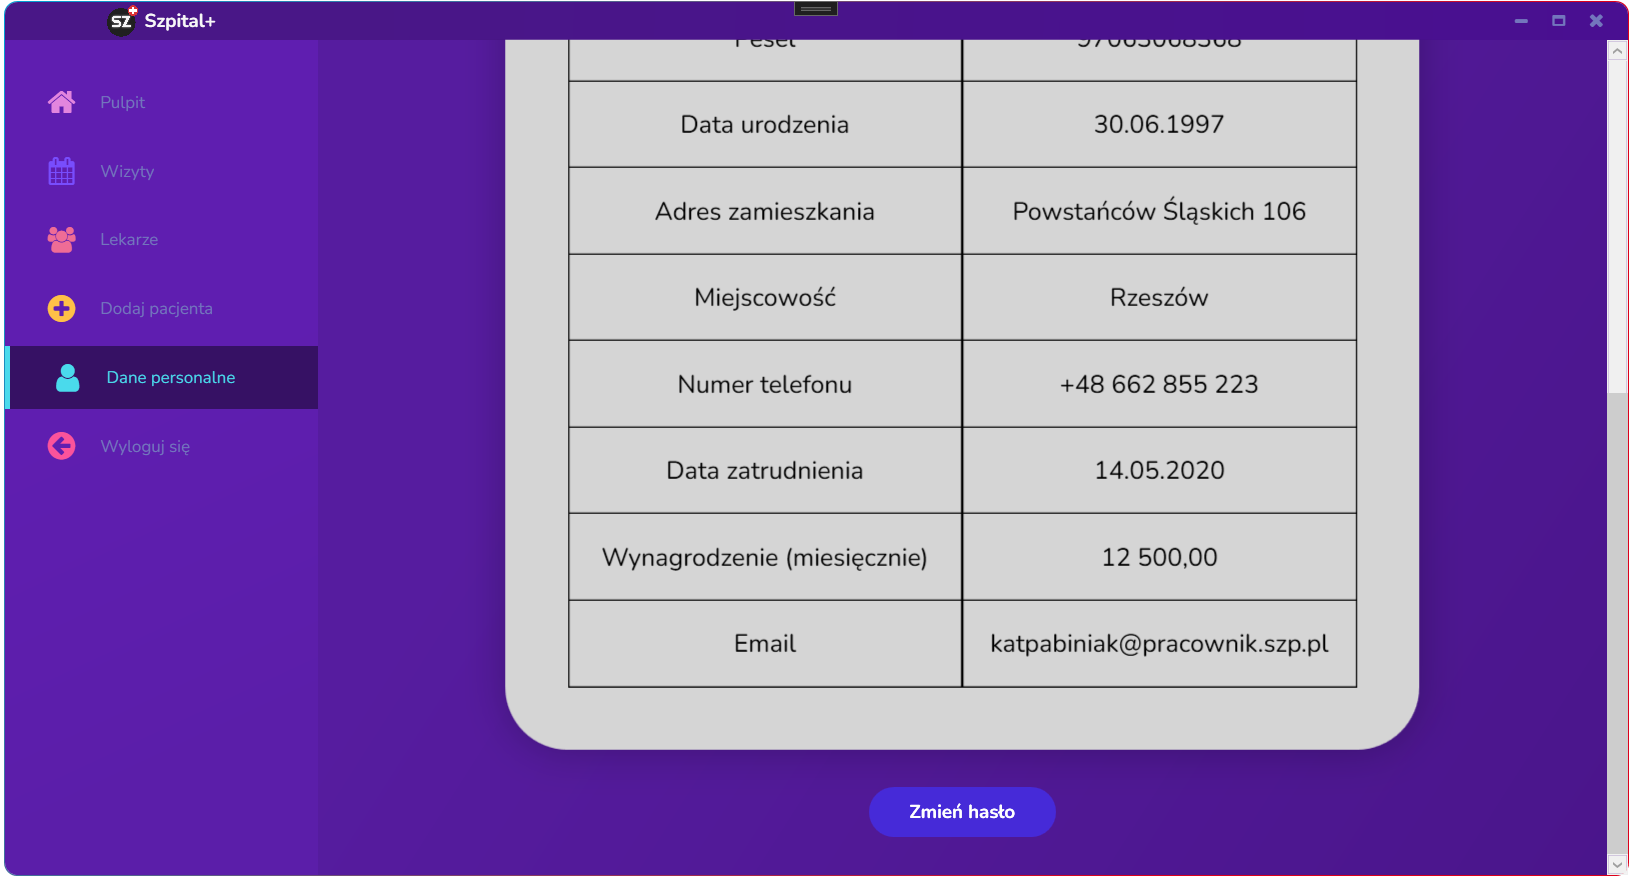
\includegraphics[width=0.7\textwidth]{images/dane_person2.png}}
    \caption{Wygląd danych personalnych}
    \label{fig:dane_person}
    \end{figure}
    \newpage
    \subsection{\Large{Zmienianie hasła}}
    \hspace{5mm}Zmienianie hasła dostępne na dołu okna Dane personalne za pomocą przycisku.
    \begin{figure}[H]
        \begin{center}
	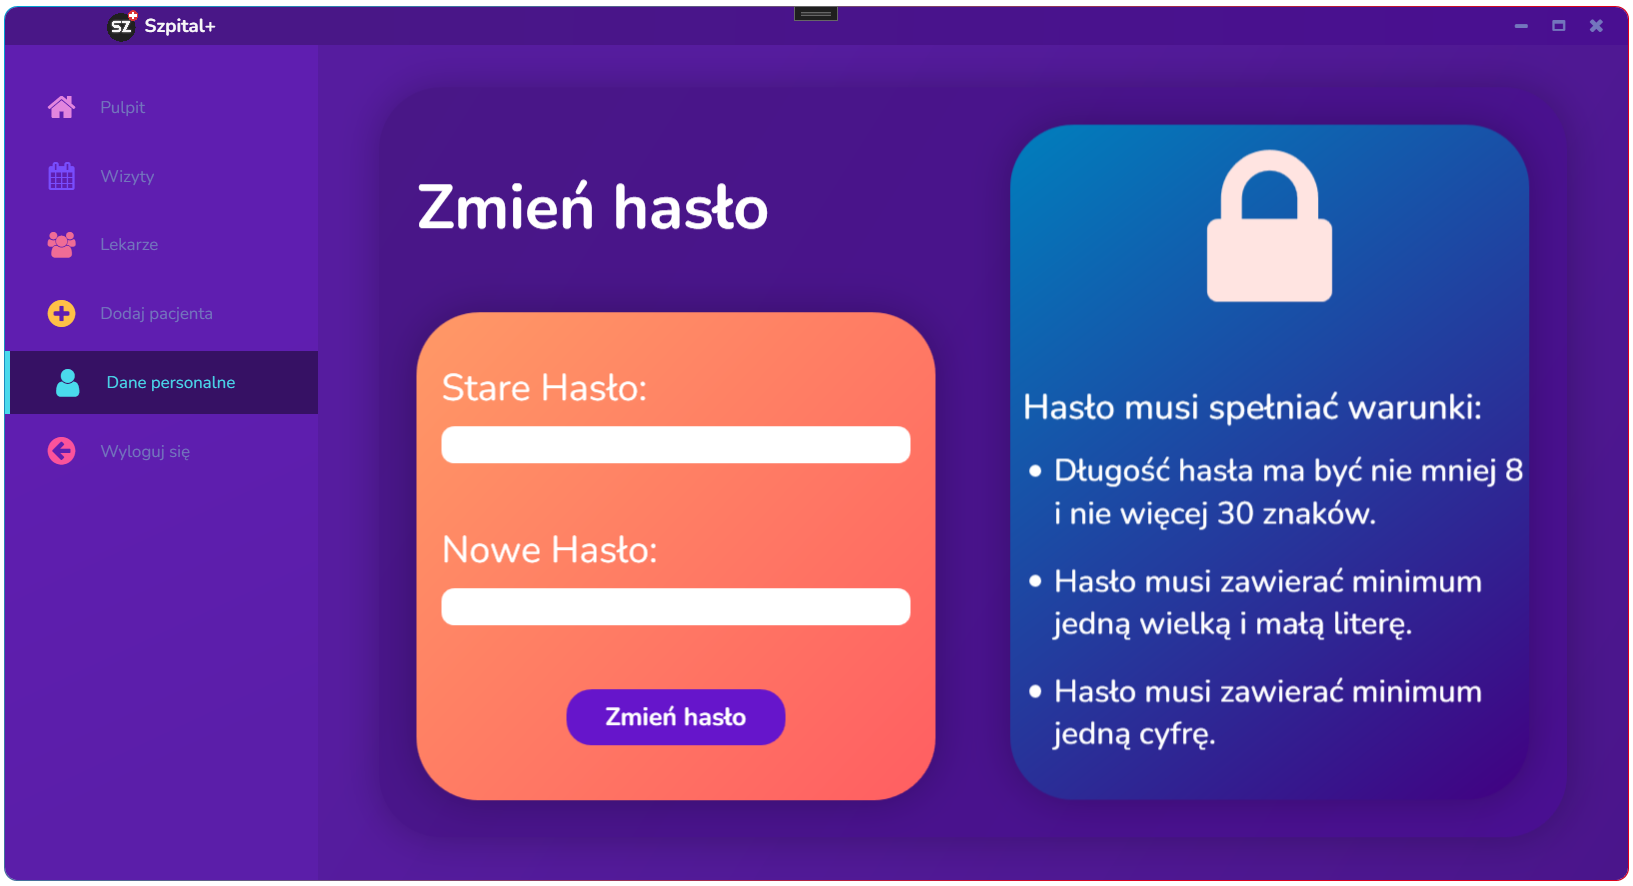
\includegraphics[height=7cm]{images/zmien_hasl.png}
        \caption{Wygląd okna \textquotedbl Zmień hasło\textquotedbl{}}
        \label{fig:zmien_hasl}
	\end{center}
    \end{figure}
    \hspace{5mm}Jeśli stare hasło nie będzie takim samym jak w bazie danych wystąpi błąd:
    \begin{figure}[H]
        \begin{center}
	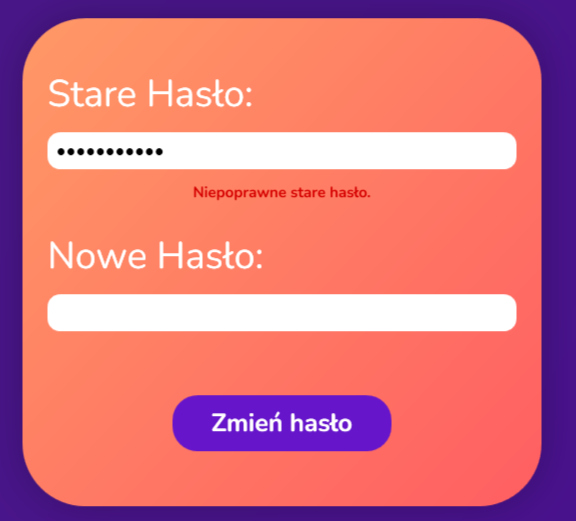
\includegraphics[height=5cm]{images/niepop_stare_hasl.png}
        \caption{Błąd przy wpisaniu starego hasła}
        \label{fig:niepop_st_haslo}
	\end{center}
    \end{figure}
    \newpage
    \subsubsection{\large{Sprawdzenie nowego hasła}}
    \hspace{5mm}Sprawdzenie nowego hasła odbywa się za pomocą {\color{blue}\href{https://en.wikipedia.org/wiki/Regular_expression}{wyrażenia regularnego}}({\color{blue}\href{https://learn.microsoft.com/en-us/dotnet/standard/base-types/regular-expression-language-quick-reference}{Klasa Regex}}).
    \begin{figure}[H]
        \begin{center}
	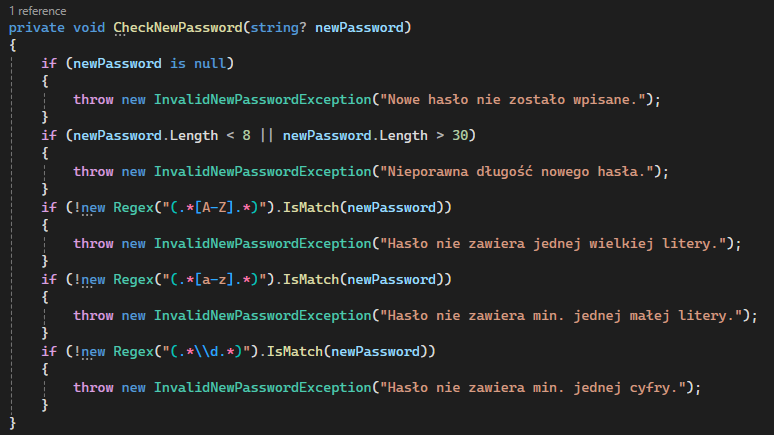
\includegraphics[height=6cm]{images/sprawdz_hasl.png}
        \caption{Metoda do sprawdzenia nowego hasła}
        \label{fig:sprawdz_hasl}
	\end{center}
    \end{figure}
    \begin{figure}[H]
        \begin{center}
	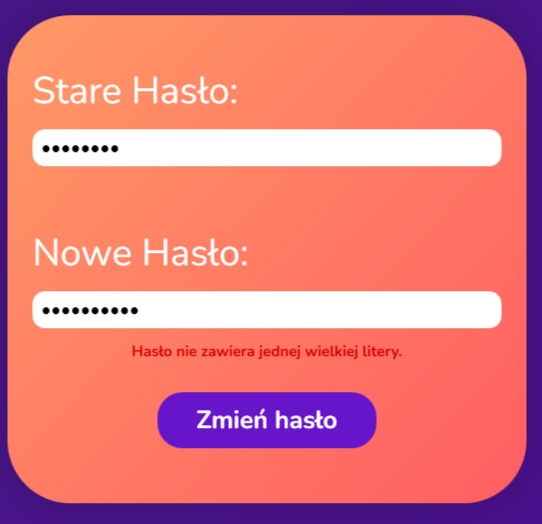
\includegraphics[height=6cm]{images/blad_nowe_hasl.png}
        \caption{Wystąpienie błędu przy nowym hasłu}
        \label{fig:blad_nowe_haslo}
	\end{center}
    \end{figure}
    \hspace{5mm}Jeśli nowe hasło odpowiada wszystkim warunkom, pojawia się okno do zatwierdzenia operacji. Przy tym interakcja z głownem oknem jest niemożliwa dopóki użykownik anuluje lub zatwierdzi operację.
    \begin{figure}[H]
        \begin{center}
	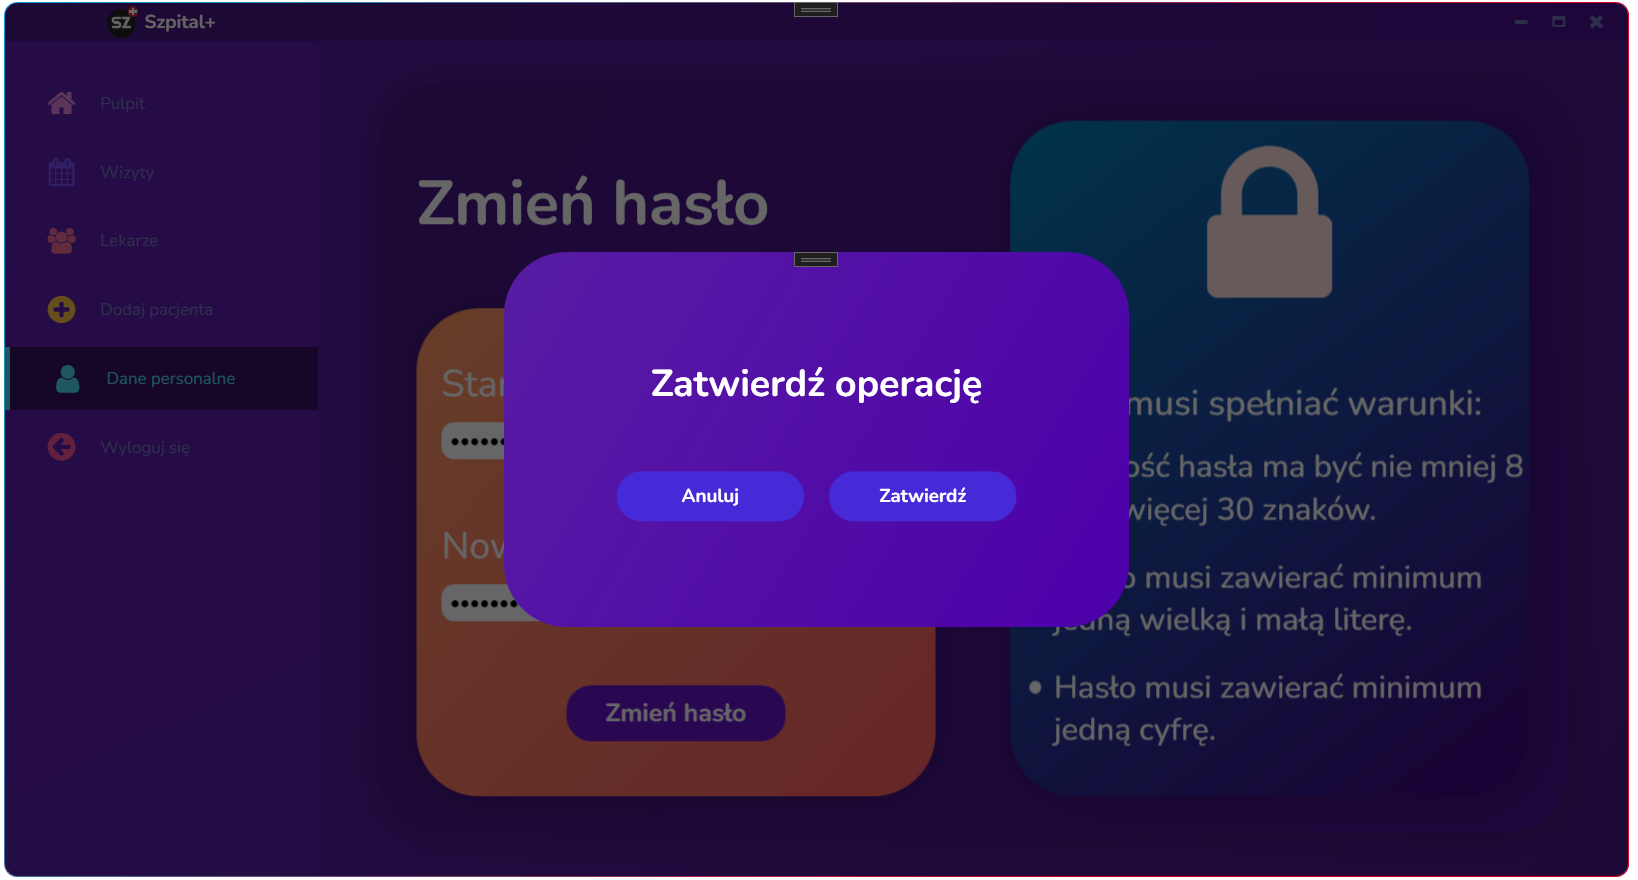
\includegraphics[height=6cm]{images/zatw_oper.png}
        \caption{Okno do zatwierdzenia operacji}
        \label{fig:zatw_oper}
	\end{center}
    \end{figure}
    \begin{figure}[H]
        \begin{center}
	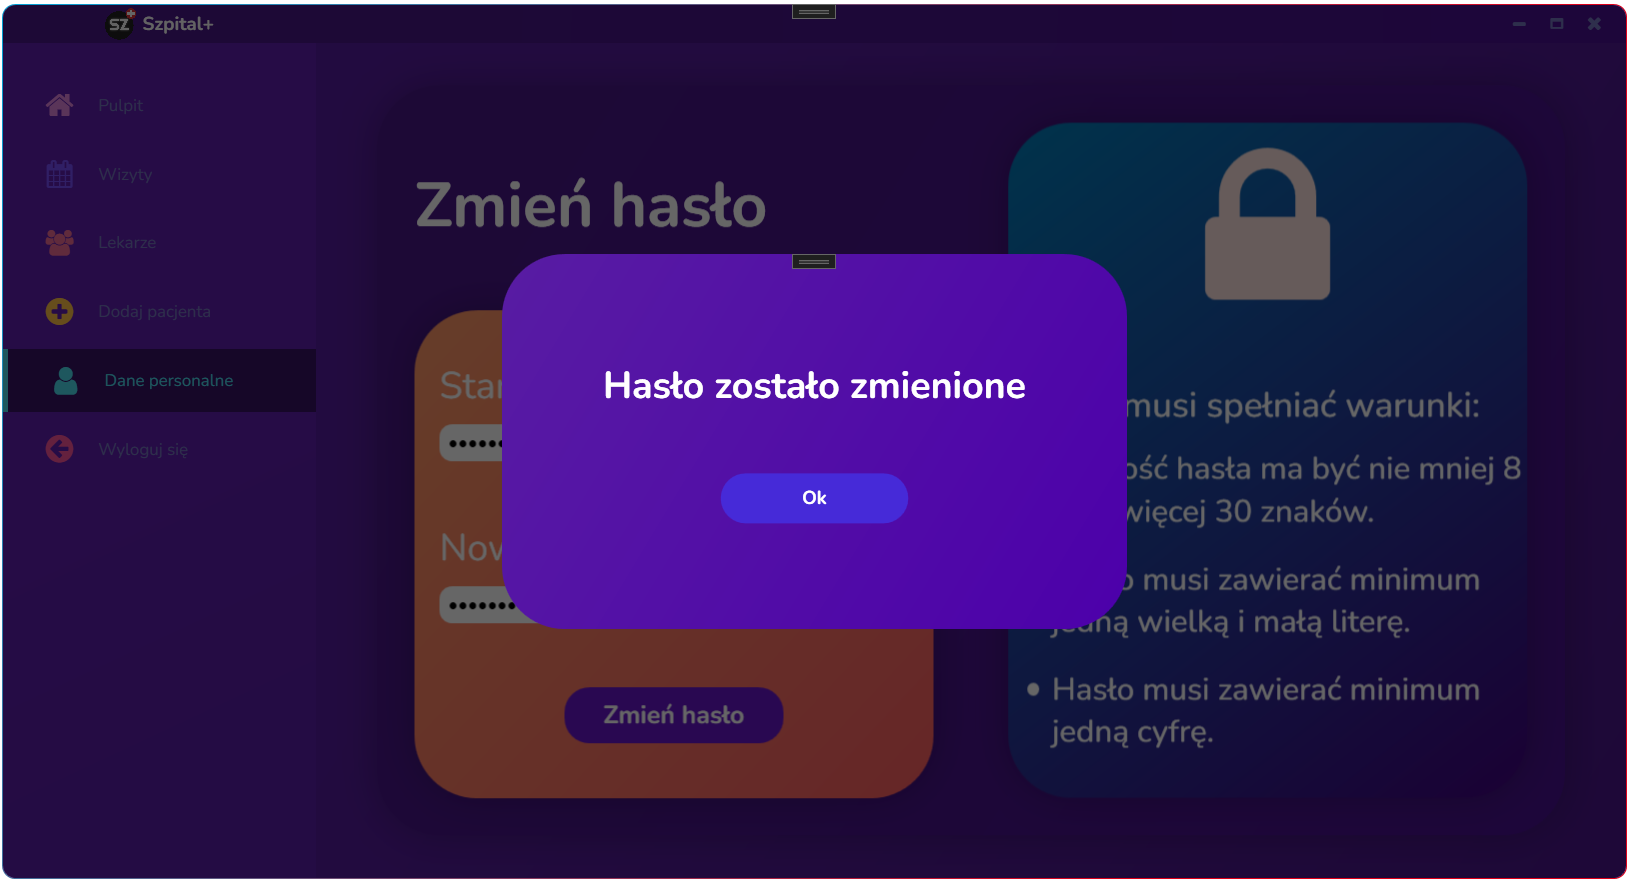
\includegraphics[height=6cm]{images/haslo_zos_zmien_katpa.png}
        \caption{Hasło zostało zmienione}
        \label{fig:haslo_zost_zmien}
	\end{center}
    \end{figure}
    \begin{figure}[H]
    \centering
    \subfigure{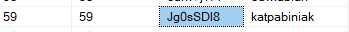
\includegraphics[width=0.4\textwidth]{images/stare_haslo_katpa.png}} 
    \subfigure{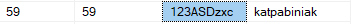
\includegraphics[width=0.4\textwidth]{images/nowe_haslo_katpa.png}}
    \caption{Nowe i stare hasło}
    \end{figure}
    \subsection{\Large{Okna dla recepcjonisty}}
    \subsubsection{\large{Wizyty - nie został zaimplementowany}}
    \subsubsection{\large{Lekarze}}
    \begin{figure}[H]
        \begin{center}
	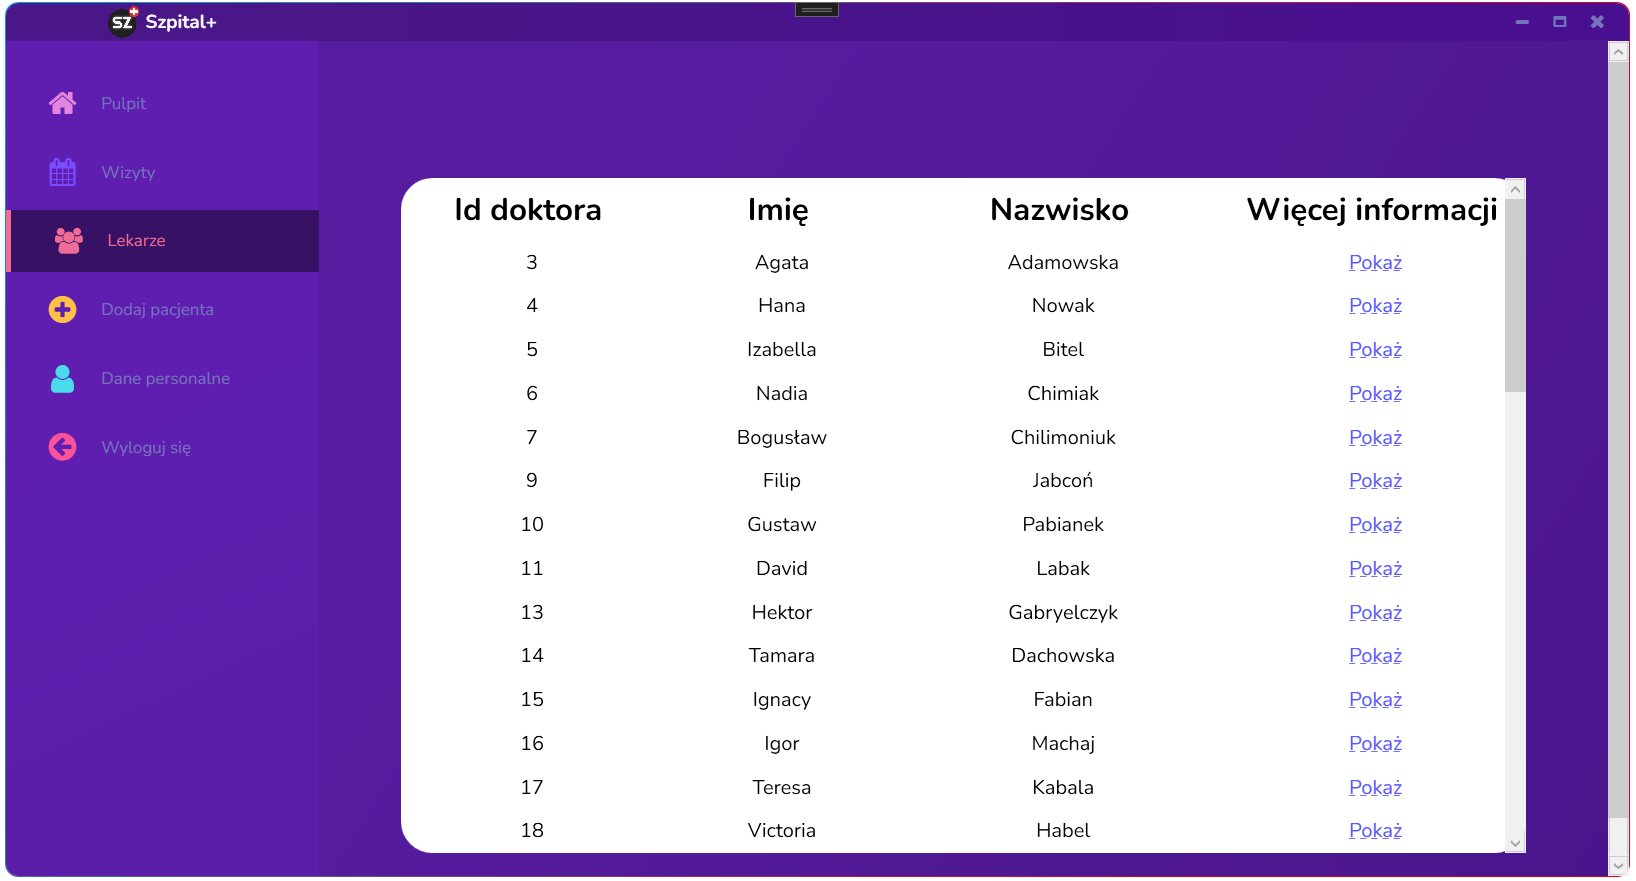
\includegraphics[height=7cm]{images/recep_lekarze.png}
        \caption{Okno recepcjonisty(Lekarze)}
        \label{fig:recep_lekarze}
	\end{center}
    \end{figure}
    \hspace{5mm}Przycisk \textquotedbl Pokaż\textquotedbl{} nie został zaimplementowany.
    \subsubsection{\large{Dodaj pacjenta}}
    \begin{figure}[H]
    \centering
    \subfigure{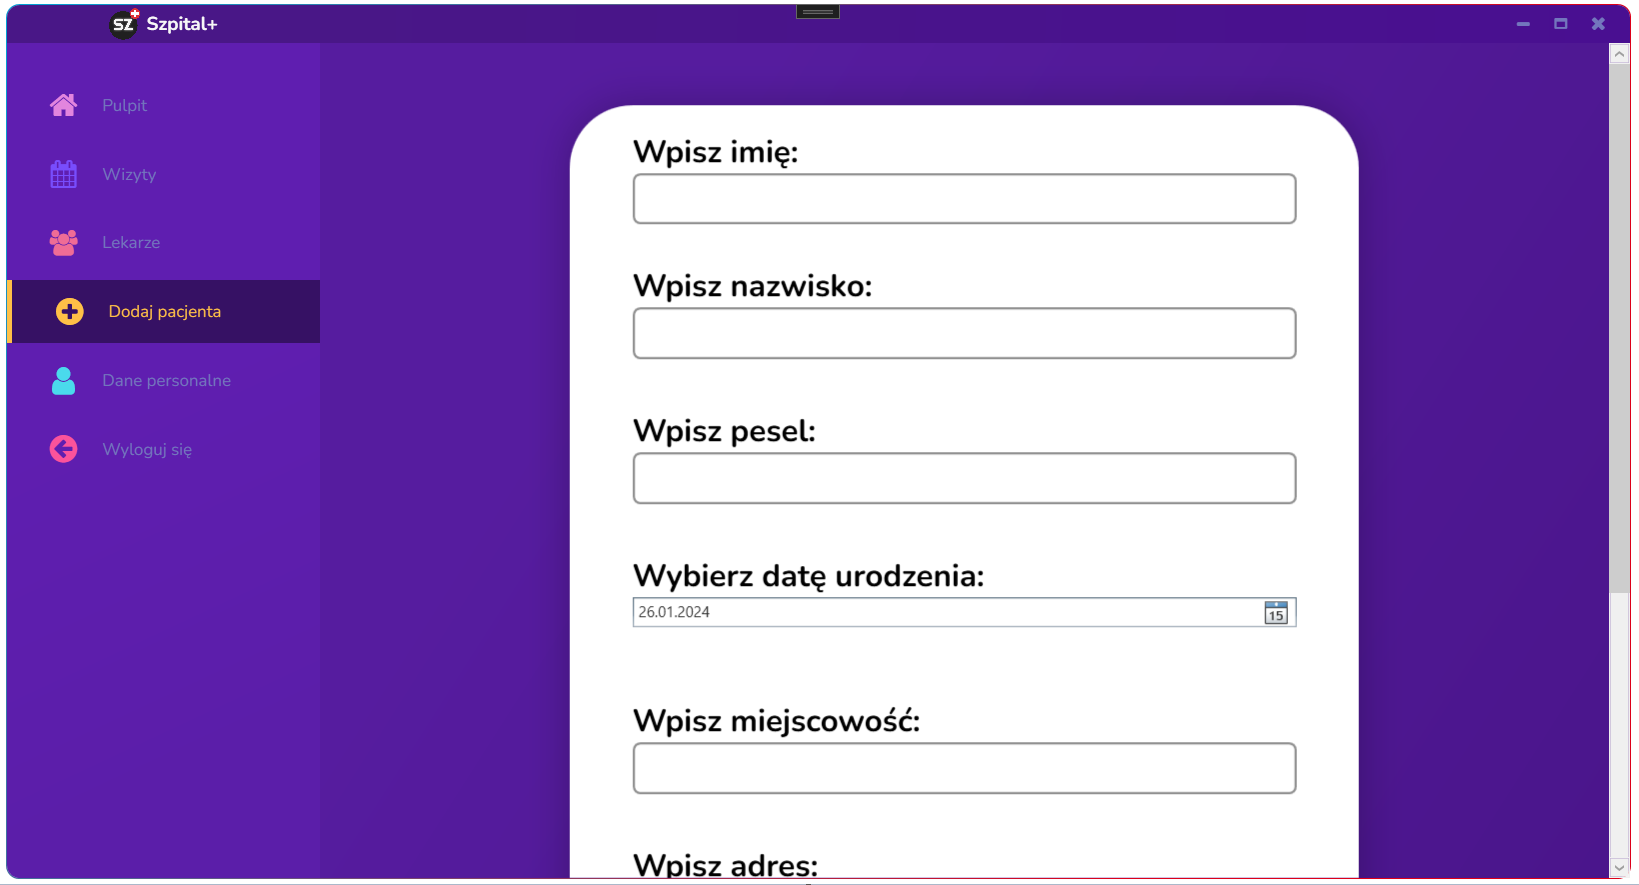
\includegraphics[width=0.5\textwidth]{images/dodaj_pacj_1.png}} 
    \subfigure{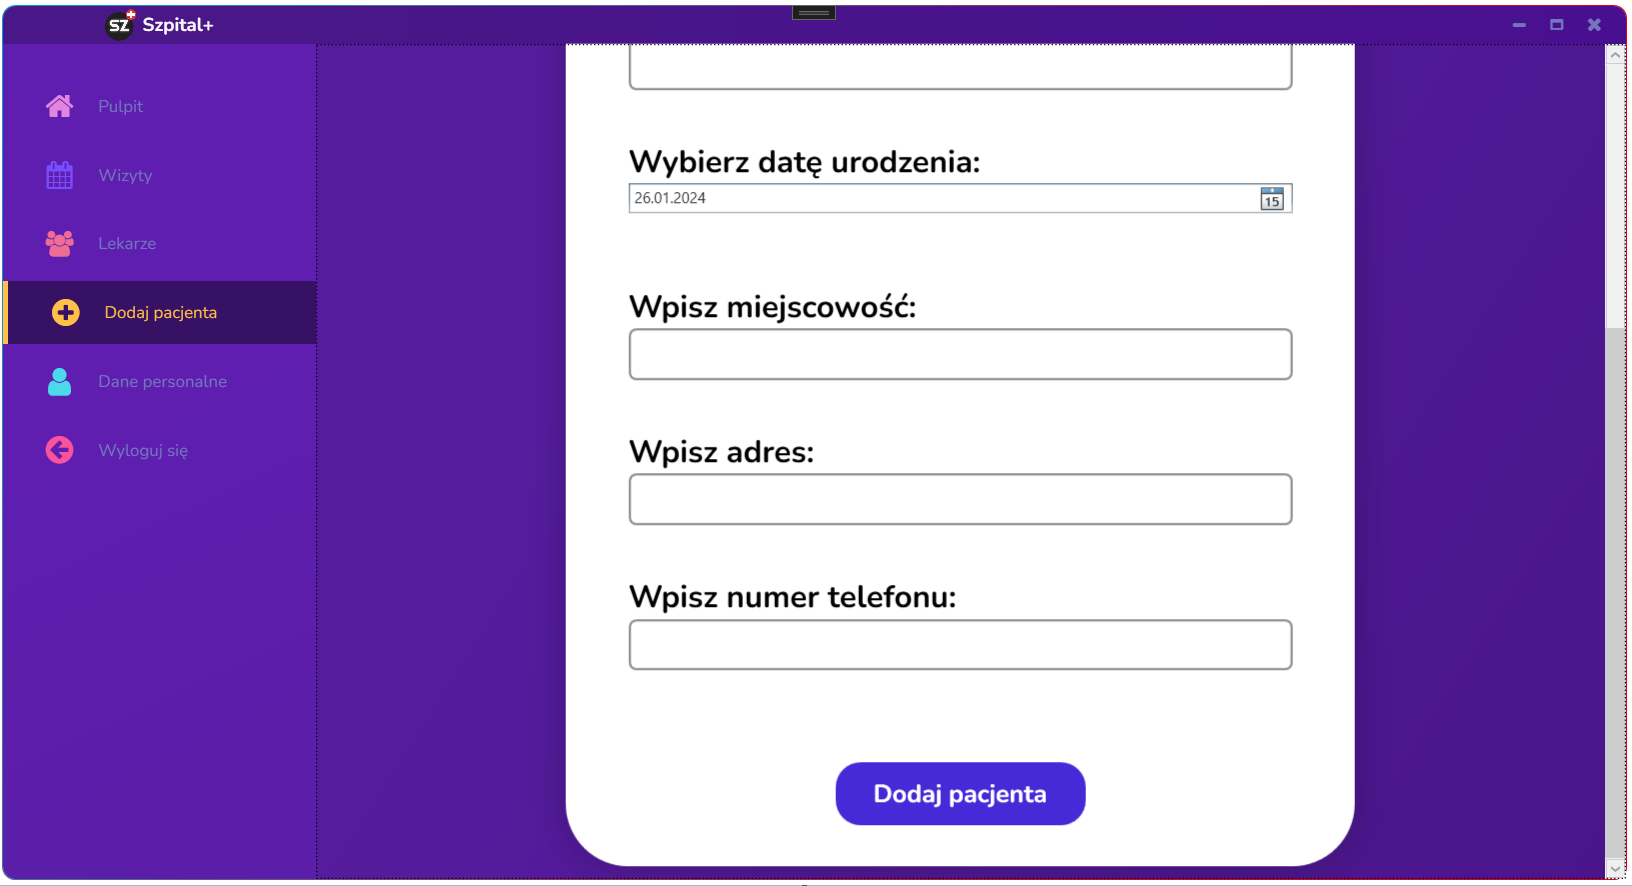
\includegraphics[width=0.5\textwidth]{images/dodaj_pacj_2.png}}
    \caption{Okno recepcjonisty(Dodaj pacjenta)}
    \end{figure}
    \begin{figure}[H]
        \begin{center}
	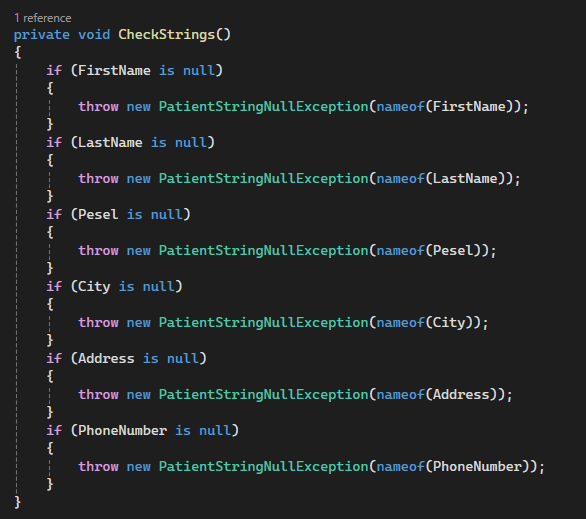
\includegraphics[height=7cm]{images/spraw_null.png}
        \caption{Sprawdzenie na puste pola}
        \label{fig:spraw_null}
	\end{center}
    \end{figure}
    \begin{figure}[H]
        \begin{center}
	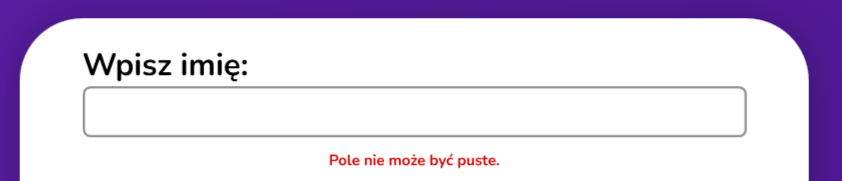
\includegraphics[height=3cm]{images/blad_wpisz_im.png}
        \caption{Wystąpienie błędu przy pustym błędzie}
        \label{fig:blad_wpisz_im}
	\end{center}
    \end{figure}
    \begin{figure}[H]
        \begin{center}
	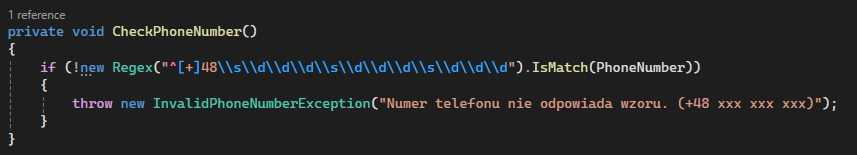
\includegraphics[height=3cm]{images/sprawd_telef.png}
        \caption{Sprawdzenie formatu telefonu}
        \label{fig:sprawd_telef}
	\end{center}
    \end{figure}
    \begin{figure}[H]
        \begin{center}
	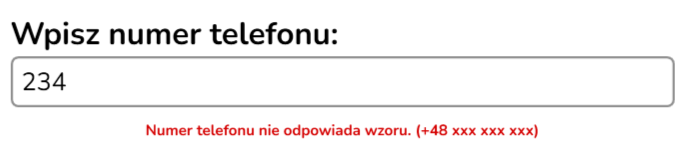
\includegraphics[height=3cm]{images/blad_telef.png}
        \caption{Błąd przy polu numeru telefonu}
        \label{fig:blad_telef}
	\end{center}
    \end{figure}
    \begin{figure}[H]
        \begin{center}
	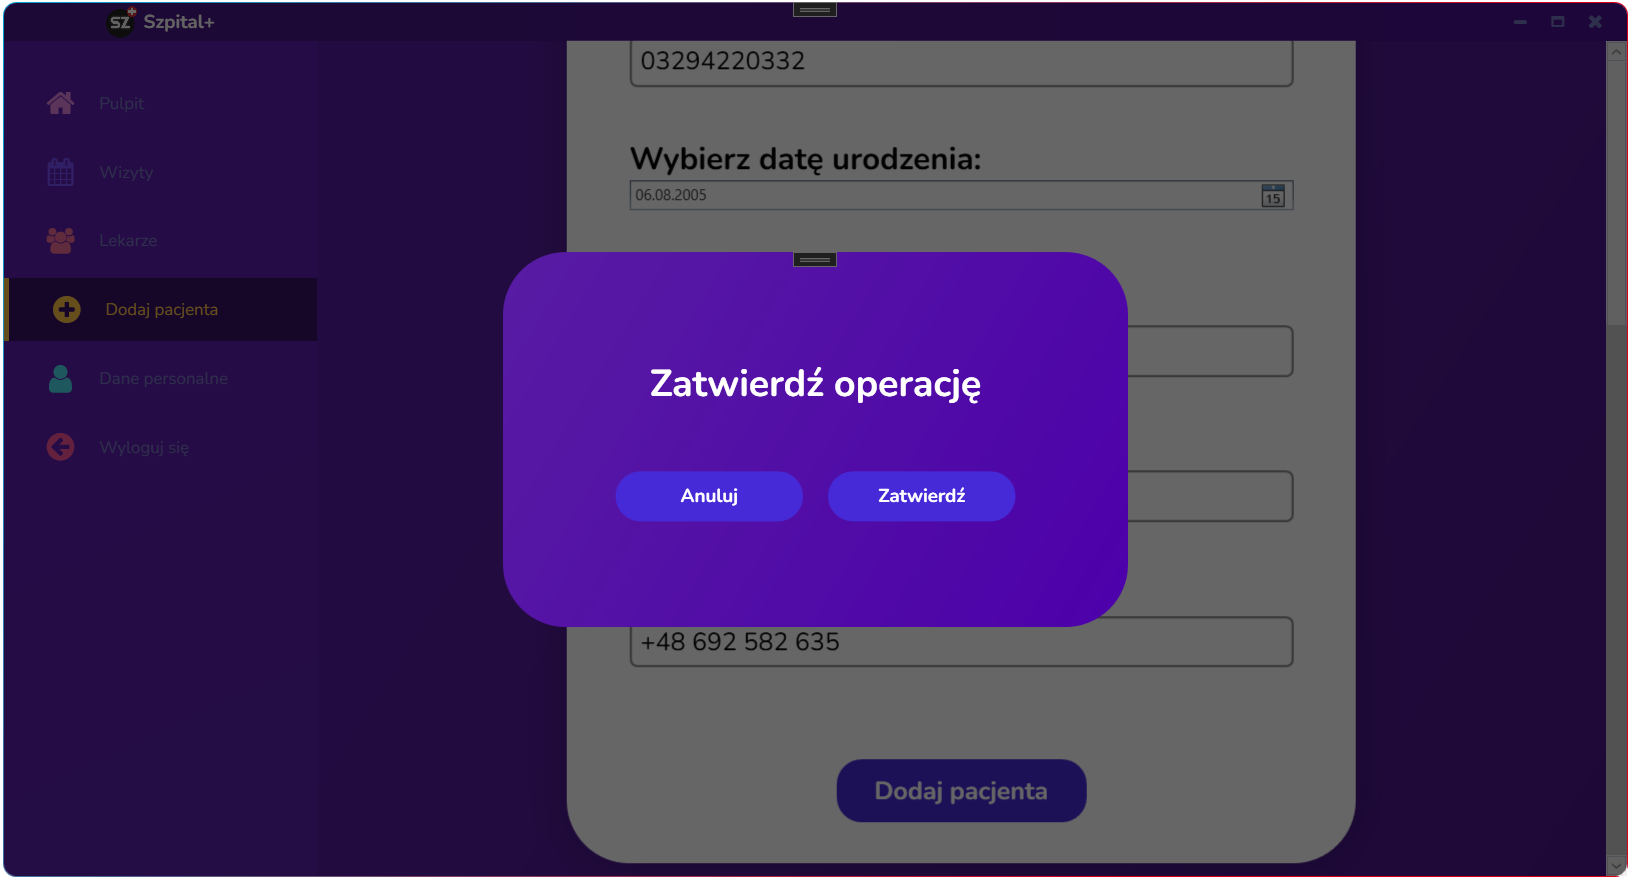
\includegraphics[height=6cm]{images/zatwr_oper_dod.png}
        \caption{Zatwierdzenie operacji}
        \label{fig:zatwr_oper_dod}
	\end{center}
    \end{figure}
    \begin{figure}[H]
        \begin{center}
	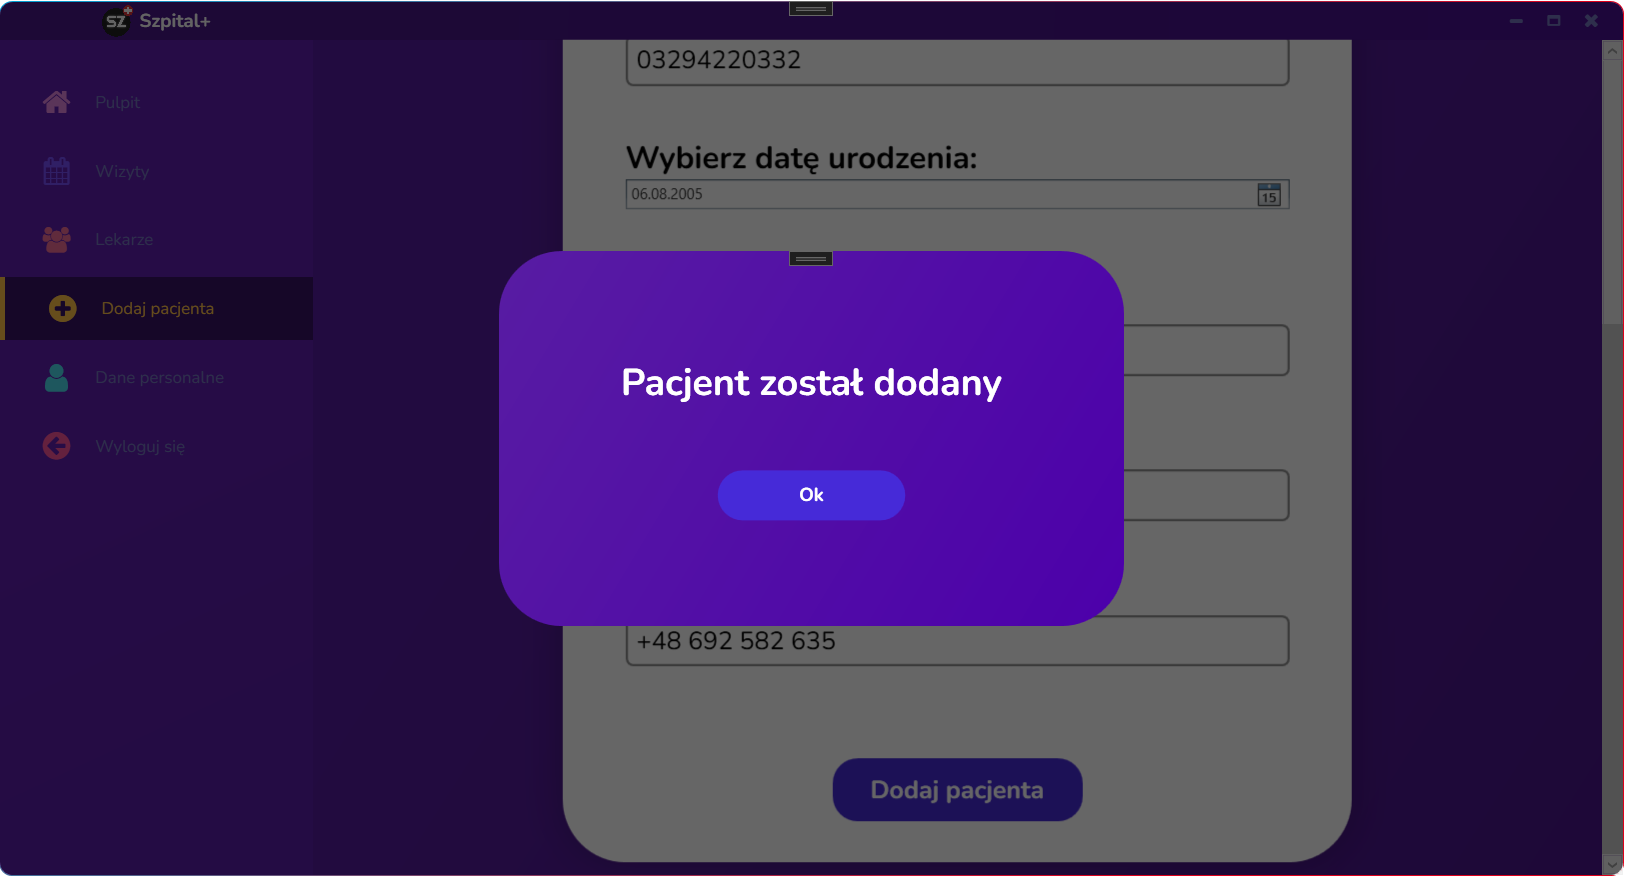
\includegraphics[height=6cm]{images/pacj_zost_dod.png}
        \caption{Pacjent został dodany}
        \label{fig:pacj_zost_dod}
	\end{center}
    \end{figure}
    \begin{figure}[H]
    \centering
    \subfigure{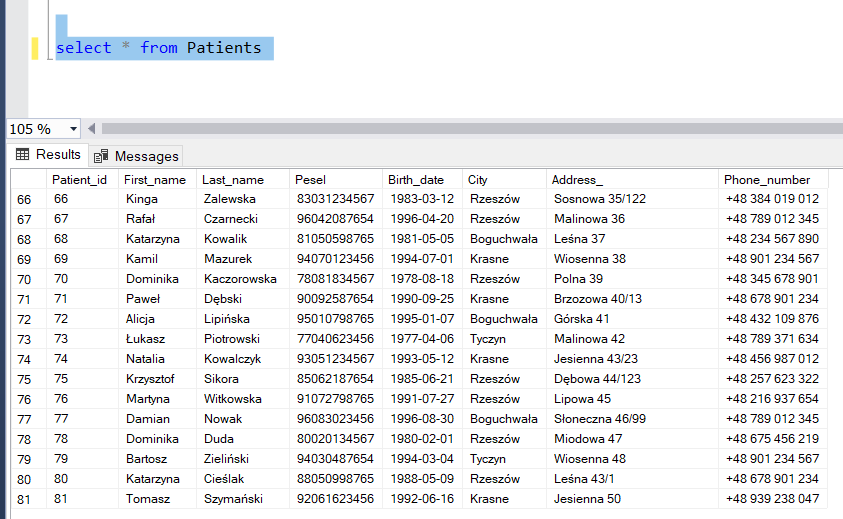
\includegraphics[width=0.6\textwidth]{images/pacjen_przed_dod.png}} 
    \subfigure{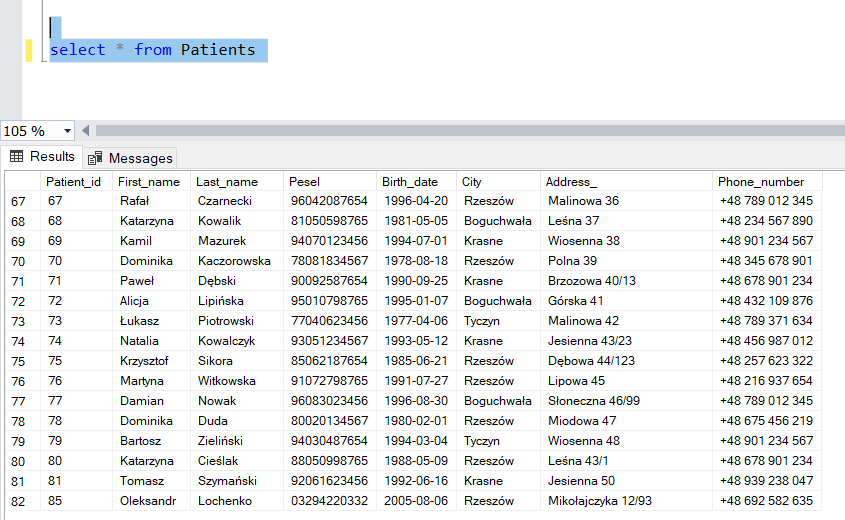
\includegraphics[width=0.6\textwidth]{images/pacjen_po_dod.png}}
    \caption{Tabela pacjentów przed i po dodaniu rekordu}
    \end{figure}

    \subsection{\Large{Okna dla głównego kierownika}}
    \subsubsection{\large{Pracownicy}}
    \begin{figure}[H]
        \begin{center}
	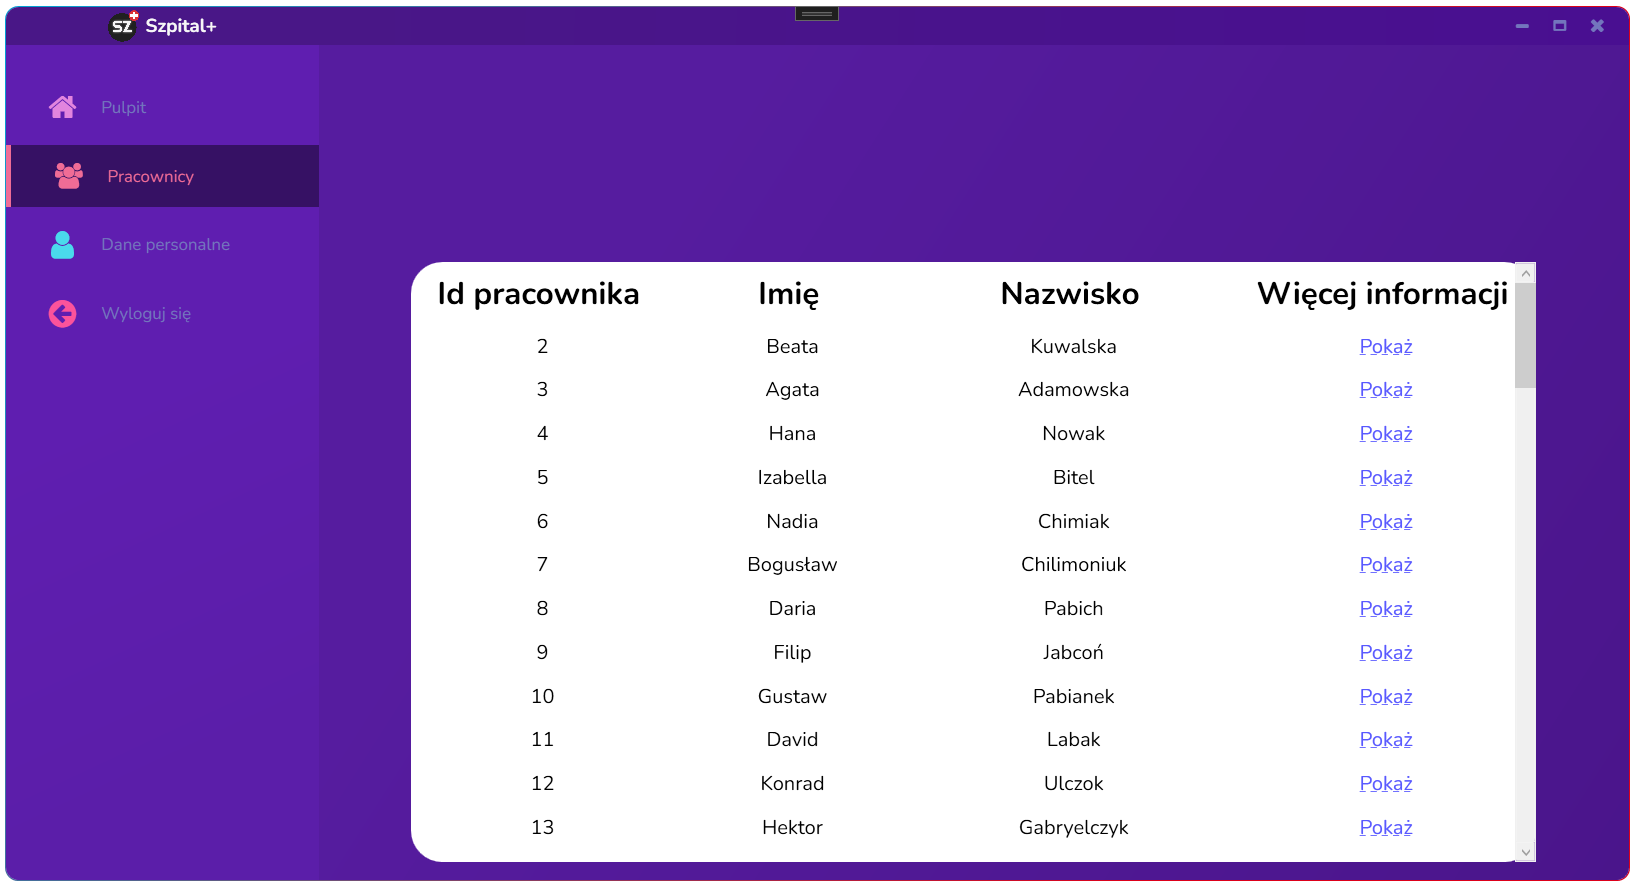
\includegraphics[height=7cm]{images/gl_kier_prac.png}
        \caption{Okno głównego kierownika(Pracownicy)}
        \label{fig:gl_kier_prac}
	\end{center}
    \end{figure}
    \hspace{5mm}Przycisk \textquotedbl Pokaż\textquotedbl{} nie został zaimplementowany.

    \subsection{\Large{Okna dla kierownika}}
    \subsubsection{\large{Lekarze}}
    \begin{figure}[H]
        \begin{center}
	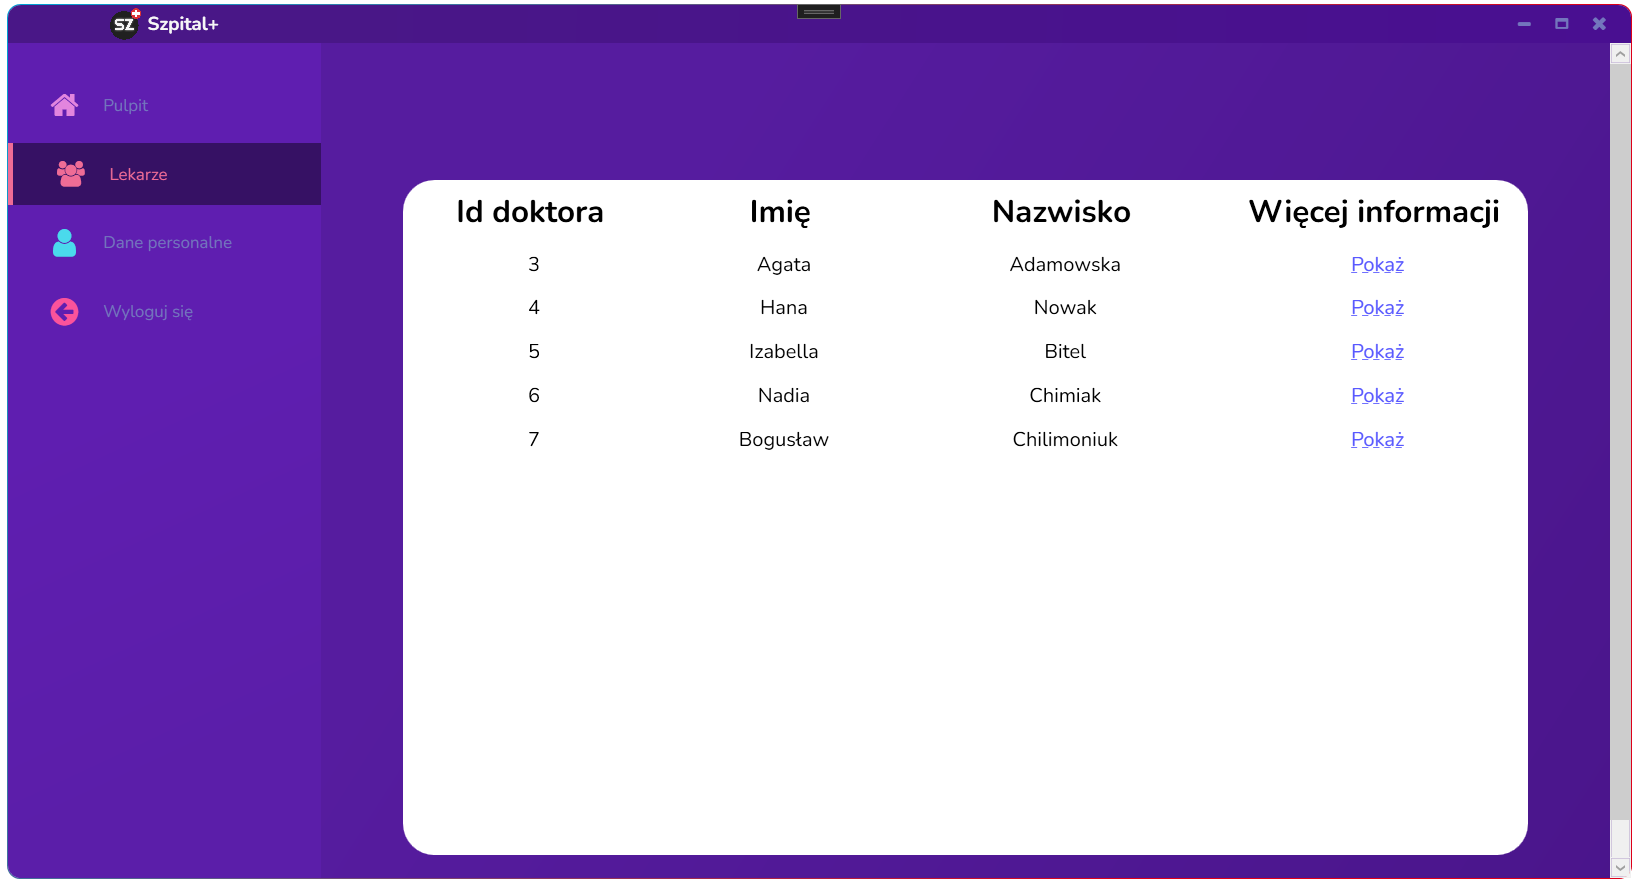
\includegraphics[height=7cm]{images/kier_lekar.png}
        \caption{Okno kierownika(Lekarze)}
        \label{fig:kier_lekar}
	\end{center}
    \end{figure}
    \hspace{5mm}Przycisk \textquotedbl Pokaż\textquotedbl{} nie został zaimplementowany.

    \subsection{\Large{Okna dla doktora}}
    \subsubsection{\large{Wizyty - nie został zaimplementowany}}
    
\end{flushleft}